\chapter{User study} \label{chapter3}

    Before the functionalities implementation process, to achieve a solution as helpful as possible, we decided to perform a study that lucidly emphasizes the needs, desires, and preferences of students. We believe such research is crucial for understanding the obstacles encountered and identifying meaningful enlightening schemes. Moreover, this examination is an ideal way to confirm that the ideas we have thought of meeting follow the requirements of students. The current thesis is based on the statement of Kurt Lewin, a former psychologist established in the United States, which mentions that “\textit{No research without action, no action without research.}”

\section{Methods} \label{3:methods}

    To obtain a satisfactory data set, we used several methods to collect various comprehensive answers.
    
    Initially, the most common approach we used for this purpose was our investigation, perception, and examination for four years. We activated both as a Bachelor's degree student at \acrshort{acs}/\acrshort{upb} and as an employee at a multinational company in Bucharest, Romania. Being a reasonably significant period, we had enough time to live different emotions and experiences. At the same time, our judgment is based on the interaction with different groups of students who have distinctive backgrounds and thoughts. Equally, we were exposed to both physical and online education systems. Therefore we can make a powerful comparison between the two.
    
    In addition, we chose to interview multiple students to discover in more detail their experiences and feelings about our faculty of choice. The main topic of these discussions was focused on collecting insights about how professors and university management perceive students. More precisely, we were interested in finding out if students consider that their opinions matter and, if so, to what extent. Likewise, our targeted students were asked for their points of view on the general importance of feedback in developing the educational process and how much they have contributed over time.
    
    Last but not least, we conducted a survey between November and December 2020, which gathered \textbf{108} answers, which represents approximately \textbf{20\%} out of the total number of students enrolled in a B.Sc. year. It was distributed as a Google Form document on several groups from social networks, both through the aid of our author and the group of Counselors and Senators Students of \acrshort{upb}.
    
    Next, throughout this chapter, we will analyze all the answers received to this form, presenting detailed statistics of the current situation at \acrshort{acs}/\acrshort{upb}.
    
\section{Target audience} \label{3:target_audience}

    The distributed questionnaire was addressed to students from any year in Bachelor's and Master's degrees, regardless of age, sex, or religious orientation.
    
    \begin{figure}[ht]
        \centering
             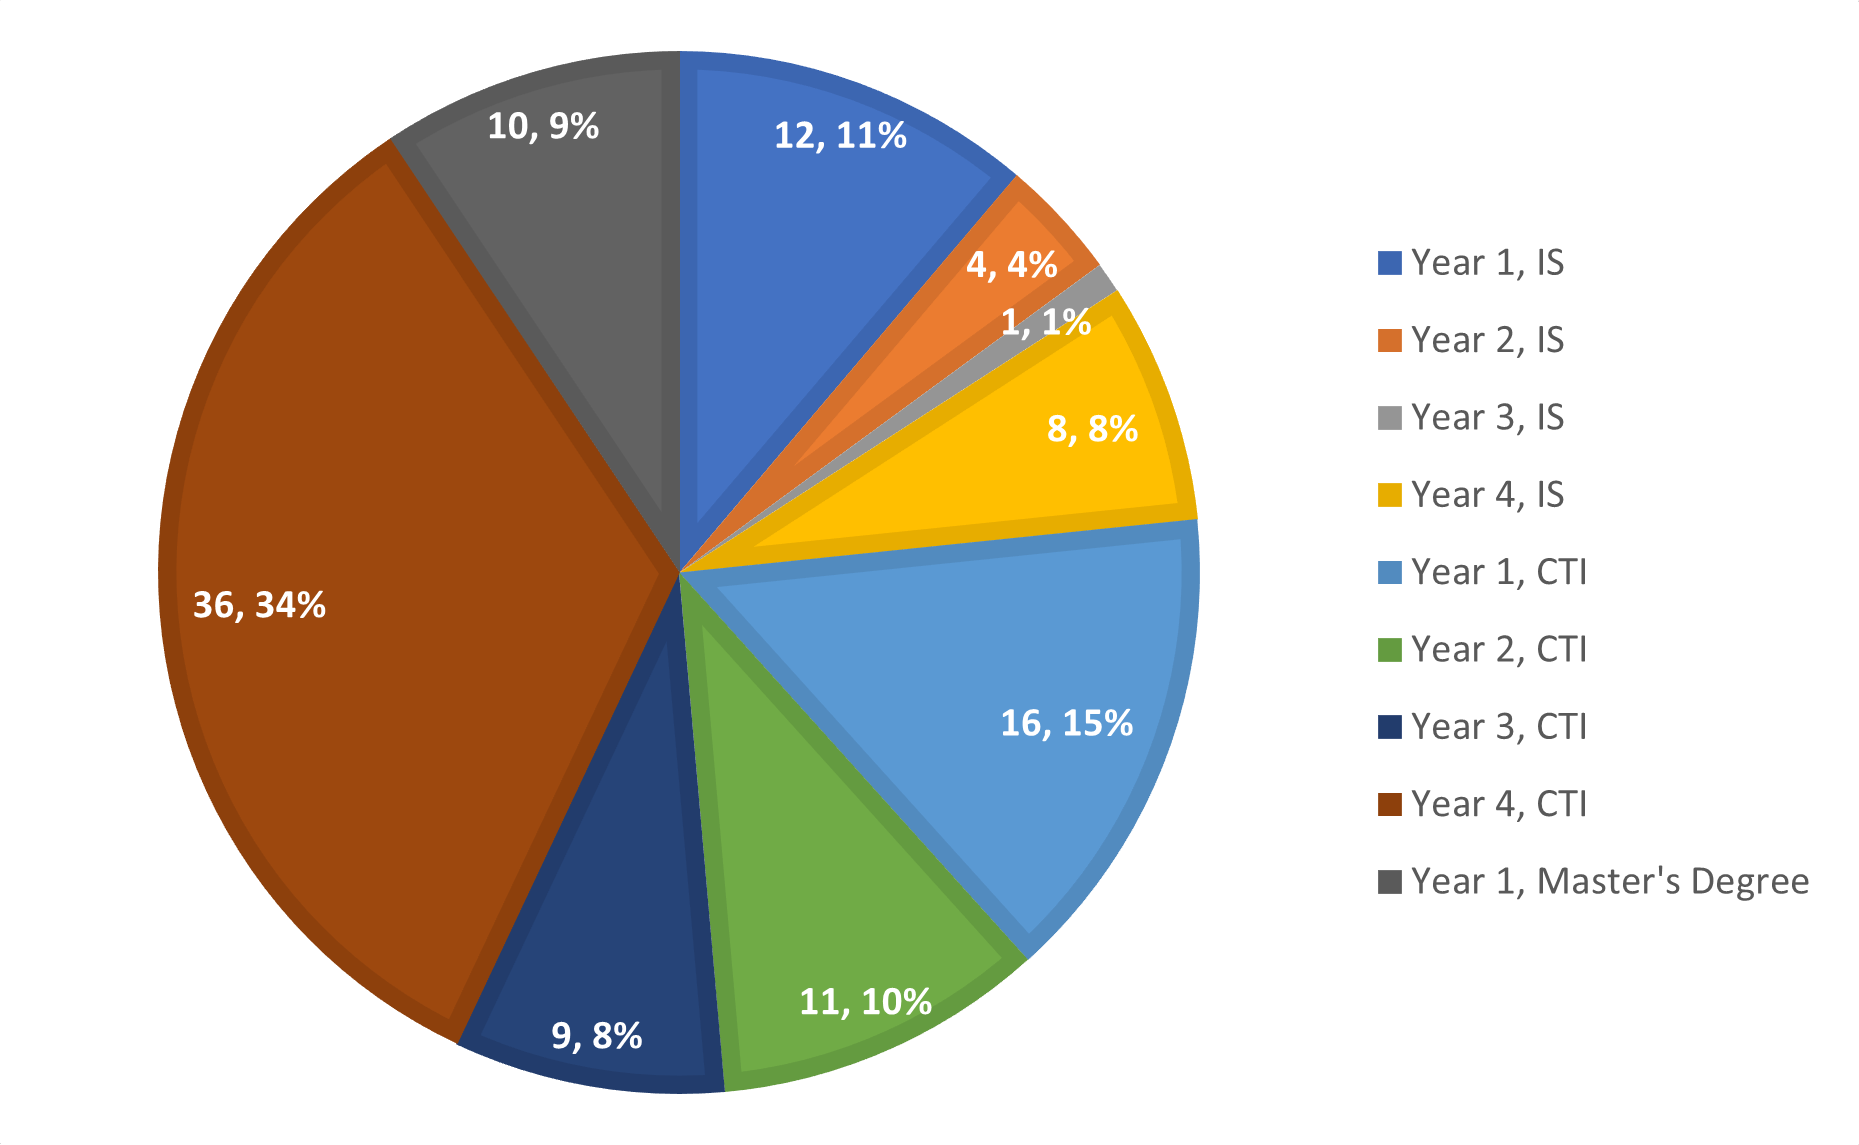
\includegraphics[height=0.3\textheight]{figures/charts/survey/students_distribution.png}
        \caption{Distribution of students according to the year of study and specialization}
        \label{3:fig:students_distribution}
    \end{figure}

    The highest percentage of responses came from students in the last year of study, B. Sc. At the same time, it is worth mentioning that about \textbf{36\%} of participants are enrolled in the Systems Engineering (IS) specialization, whereas \textbf{54\%} follow the Computers and Information Technology (CTI) department studies. In comparison, the remaining \textbf{10\%} come from various Master's degrees.

\section{Results} \label{3:results}

    We noticed that about half of the total number of students interested in feedback does not always share ideas and thoughts, as seen in figure \ref{3:fig:feedback_distribution}. Therefore, students should be encouraged not to disregard this process, always keeping in mind that their opinions can contribute to the better development of the educational system.
    
    \begin{figure}[ht]
        \centering
             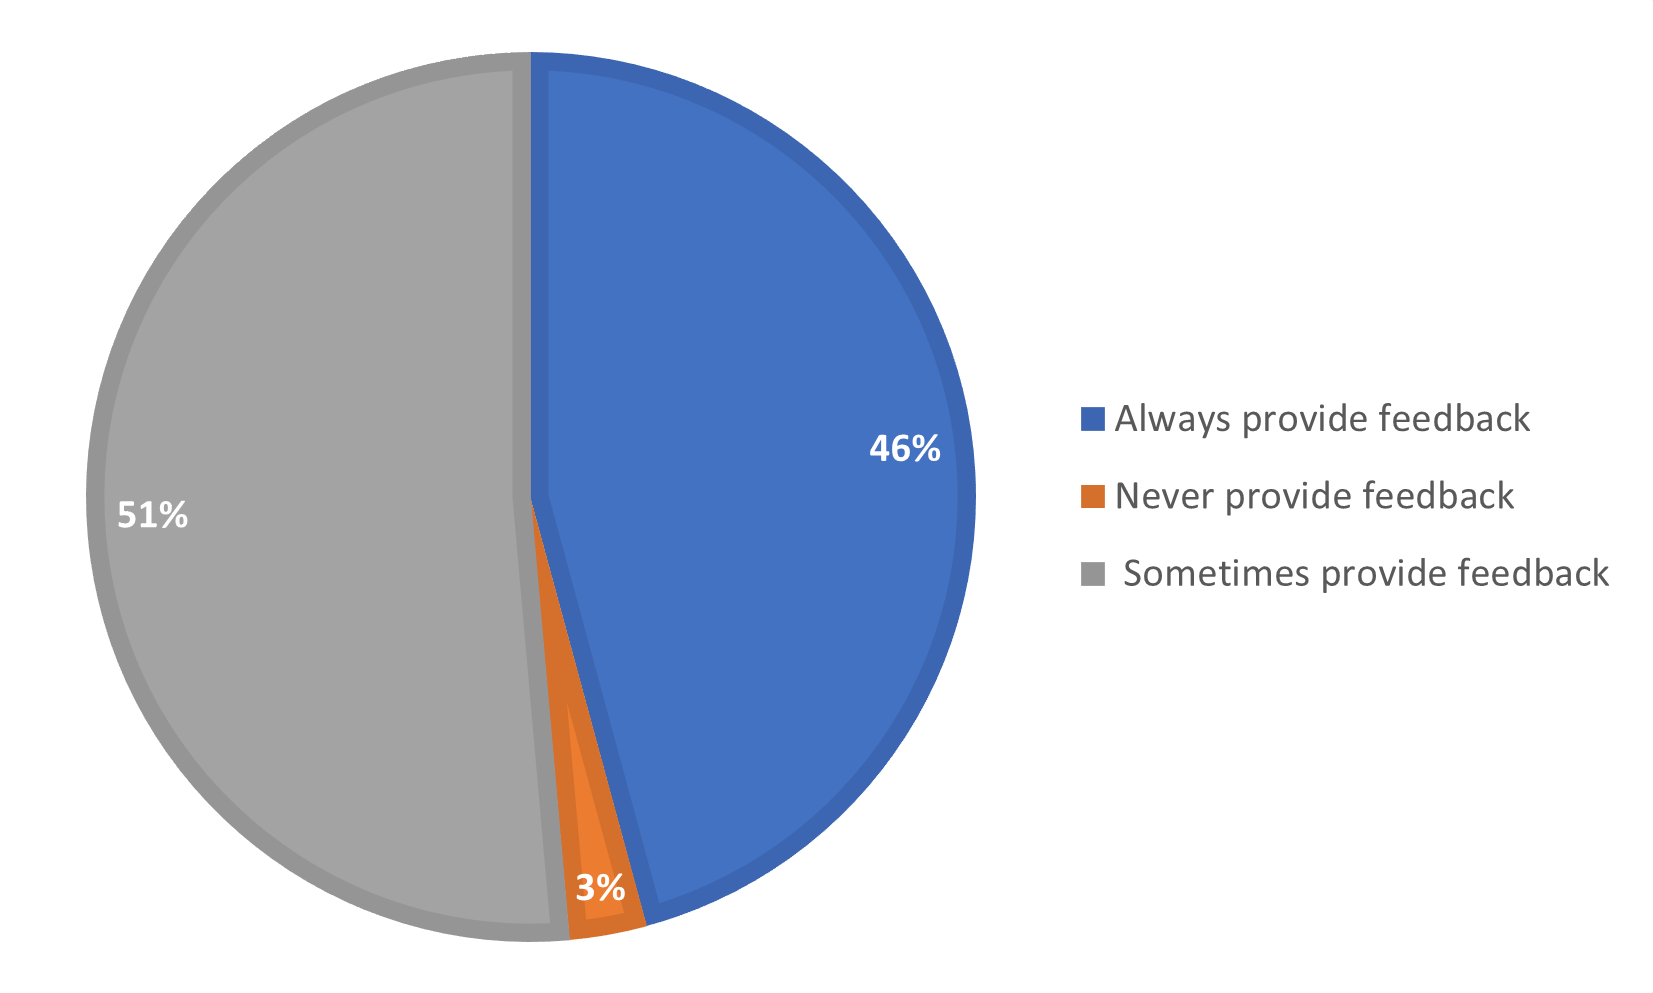
\includegraphics[height=0.25\textheight]{figures/charts/survey/feedback_distribution.png}
        \caption{Distribution of students who provide feedback or not}
        \label{3:fig:feedback_distribution}
    \end{figure}
    
    Regarding students who always provide feedback, most prefer to use the official Moodle platform and other official forms made by teachers. These statistics are also maintained in case students choose to provide occasional feedback:
    
    \clearpage
    
    \begin{figure}[ht]
        \centering
             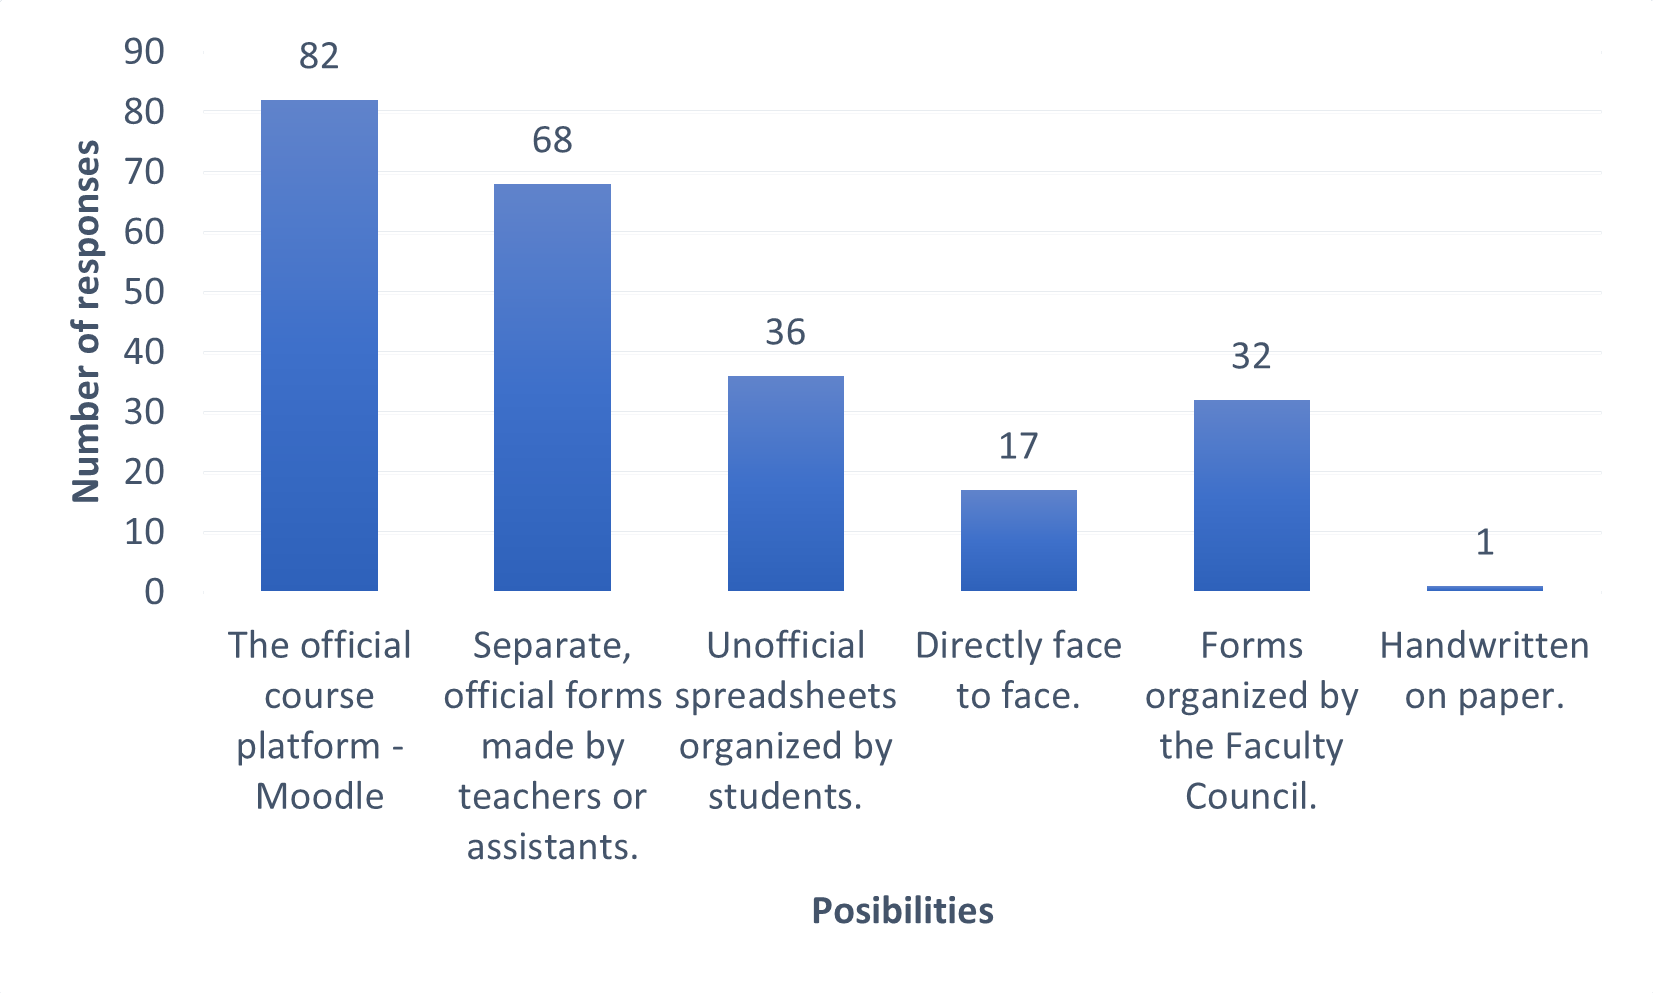
\includegraphics[height=0.322\textheight]{figures/charts/survey/feedback_platforms.png}
        \caption{Platforms and methods used for sharing feedback}
        \label{3:fig:feedback_platforms}
    \end{figure}
    
    In addition, the main reasons for providing feedback are expressed in figure \ref{3:fig:reasons_feedback}:
    
    \begin{figure}[ht]
        \centering
             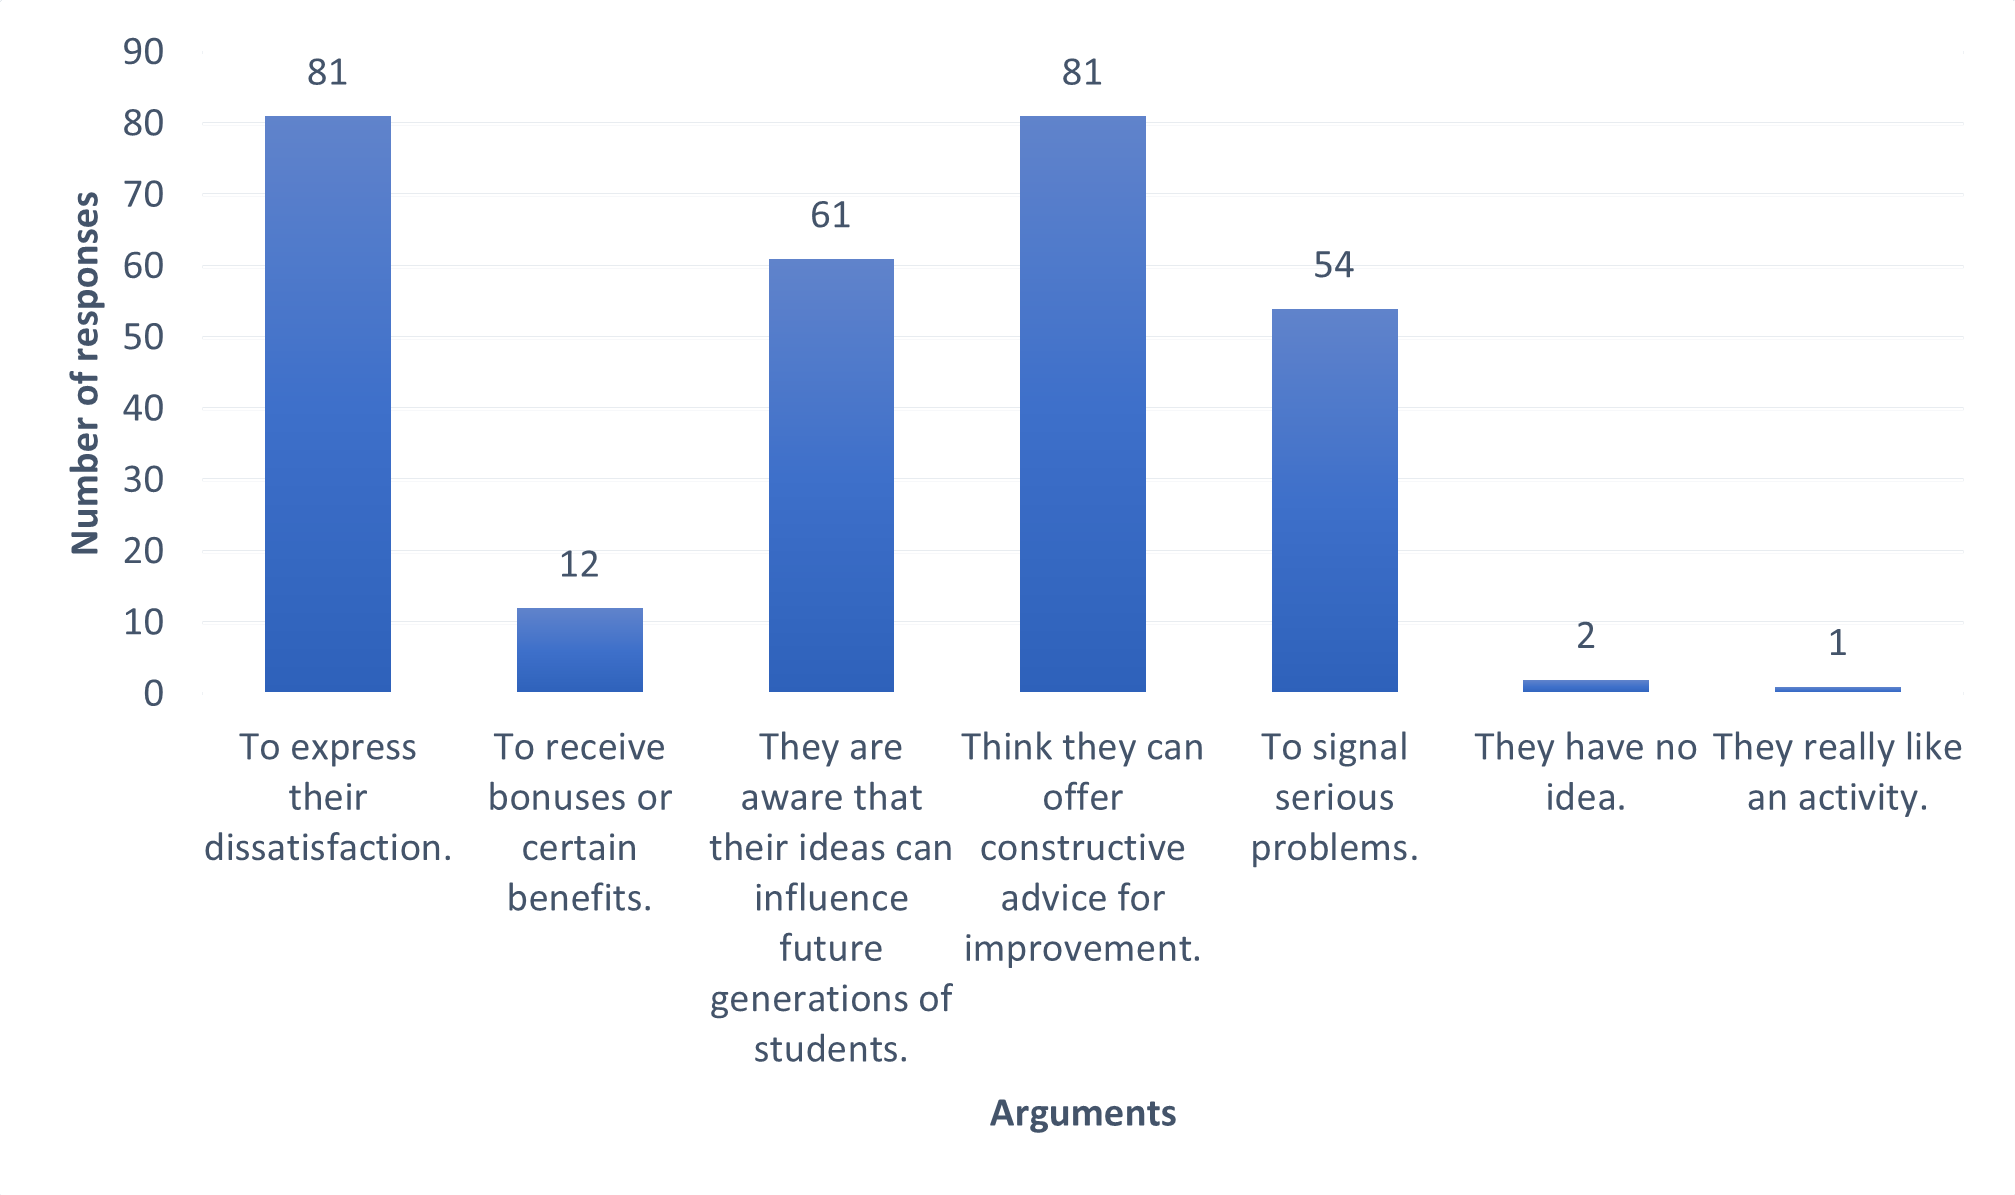
\includegraphics[height=0.322\textheight]{figures/charts/survey/reasons_feedback.png}
        \caption{Reasons why students provide feedback}
        \label{3:fig:reasons_feedback}
    \end{figure}

    Thus, \textbf{75\%} voted for both expressing dissatisfaction and thinking they can offer constructive advice for improvement. Only \textbf{11.1\%} acknowledged that they provide feedback to receive bonuses or rewards, which is a positive and gratifying aspect.
    
    As expected, most students prefer to remain anonymous when sharing their thoughts or think very well before publishing their names (fig. \ref{3:fig:feedback_anonymity}). As a result, guaranteeing anonymity and indicating how it is achieved represents an essential aspect of such an application.
    
    \begin{figure}[ht]
        \centering
             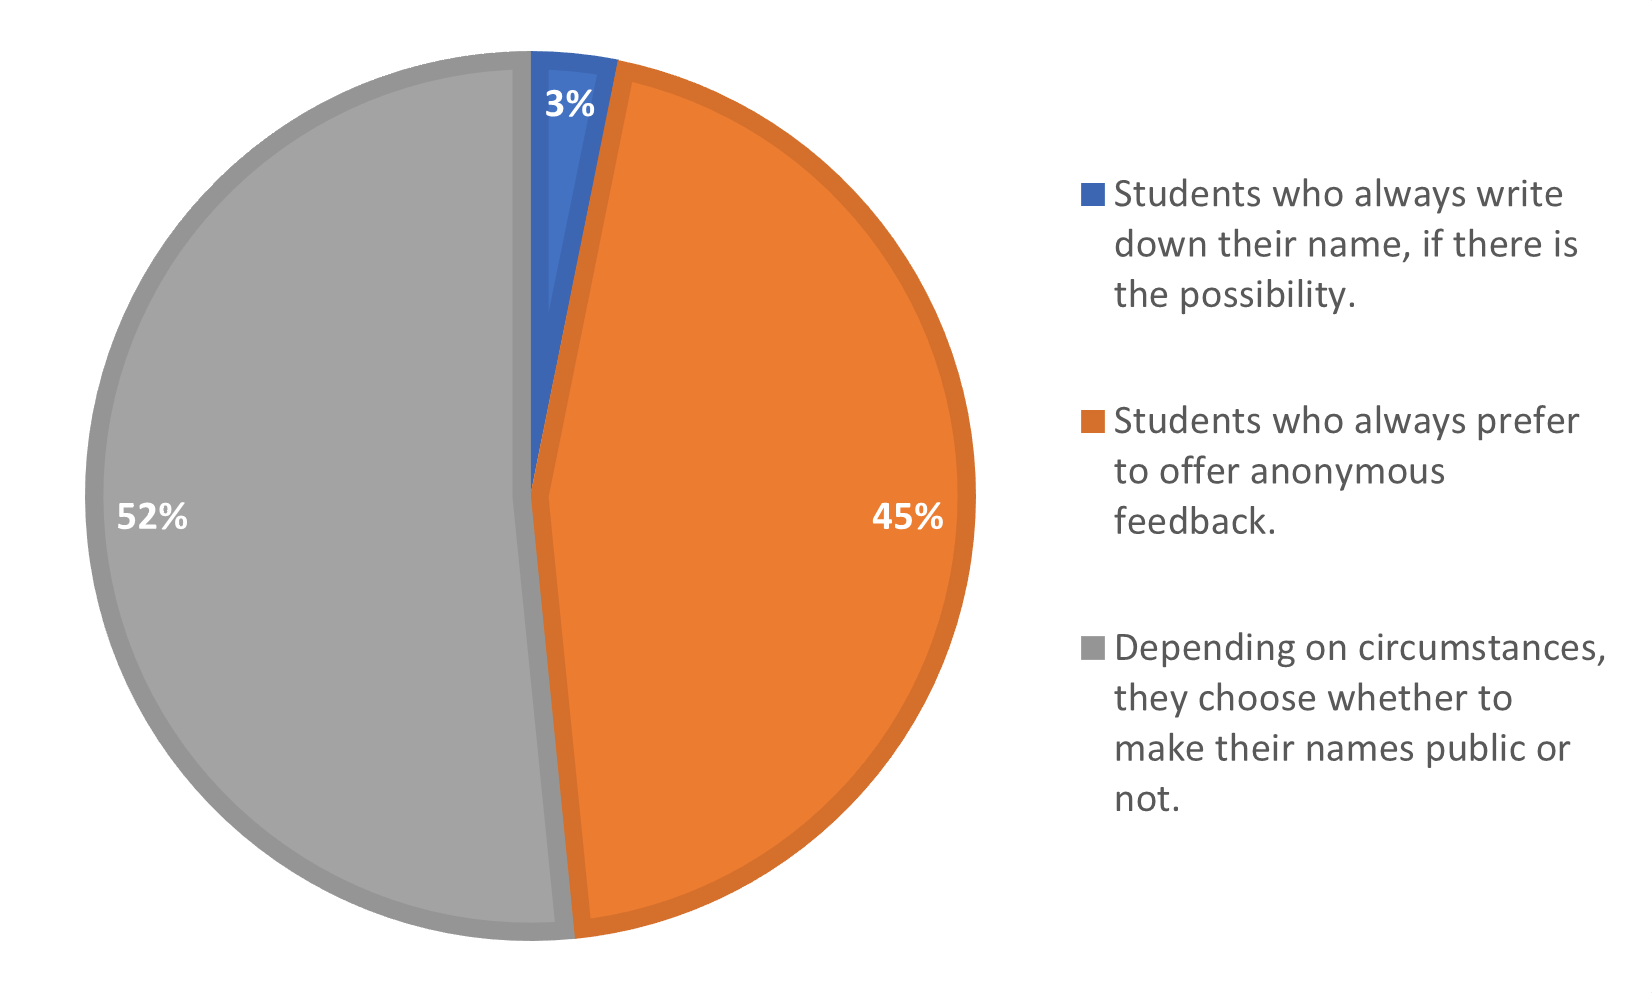
\includegraphics[height=0.25\textheight]{figures/charts/survey/feedback_anonymity.png}
        \caption{Feedback - anonymous or not?}
        \label{3:fig:feedback_anonymity}
    \end{figure}
    
    Some ideas that could help create a suitable anonymous environment are:
    
    \begin{itemize}
            \setlength{\topsep}{0.5pt}
            \setlength{\itemsep}{0.5pt}
            \setlength{\parsep}{0.5pt}
            \item feedback boxes or surveys: before being completed, the application may ask students to log out of their account
            \item using external third-party applications and websites. Many such platforms are implemented, offering many possibilities precisely because feedback is beneficial and vital in society. For instance, some examples of such websites are \textit{polleverywhere.com}, \textit{vevox.com}, \textit{freesuggestionbox.com}, \textit{surveymonkey.com}, or \textit{incognea.to}. These platforms are all free to use, and in addition, some of them also have the option to chat anonymously.
    \end{itemize}
    
    Universities might use the following methods to increase the ways of providing feedback, in combination with gamification features:
    
    \begin{itemize}
            \setlength{\topsep}{0.5pt}
            \setlength{\itemsep}{0.5pt}
            \setlength{\parsep}{0.5pt}
            \item daily pulse check-ins: display a small pop-up on the screen and ask students how are they feeling, simply by pressing a facial expression corresponding to their condition
            \item short questions to check the satisfaction level of students
            \item boxes where students can share their daily impressions about a specific topic
    \end{itemize}
    
    In general, most students decide to spend between \textbf{1} and \textbf{5} minutes filling out a form (fig. \ref{3:fig:feedback_time}). Moreover, considering that each semester has about 6-7 different classes, providing feedback needs to be simplified to ensure increased participation.
    
    Equally, another solution might be represented by the idea of not overlapping all the forms at the same time. Otherwise, an overhead might arise, which could also lead to complete abandonment.
    
    ~
    
    \begin{figure}[ht]
        \centering
             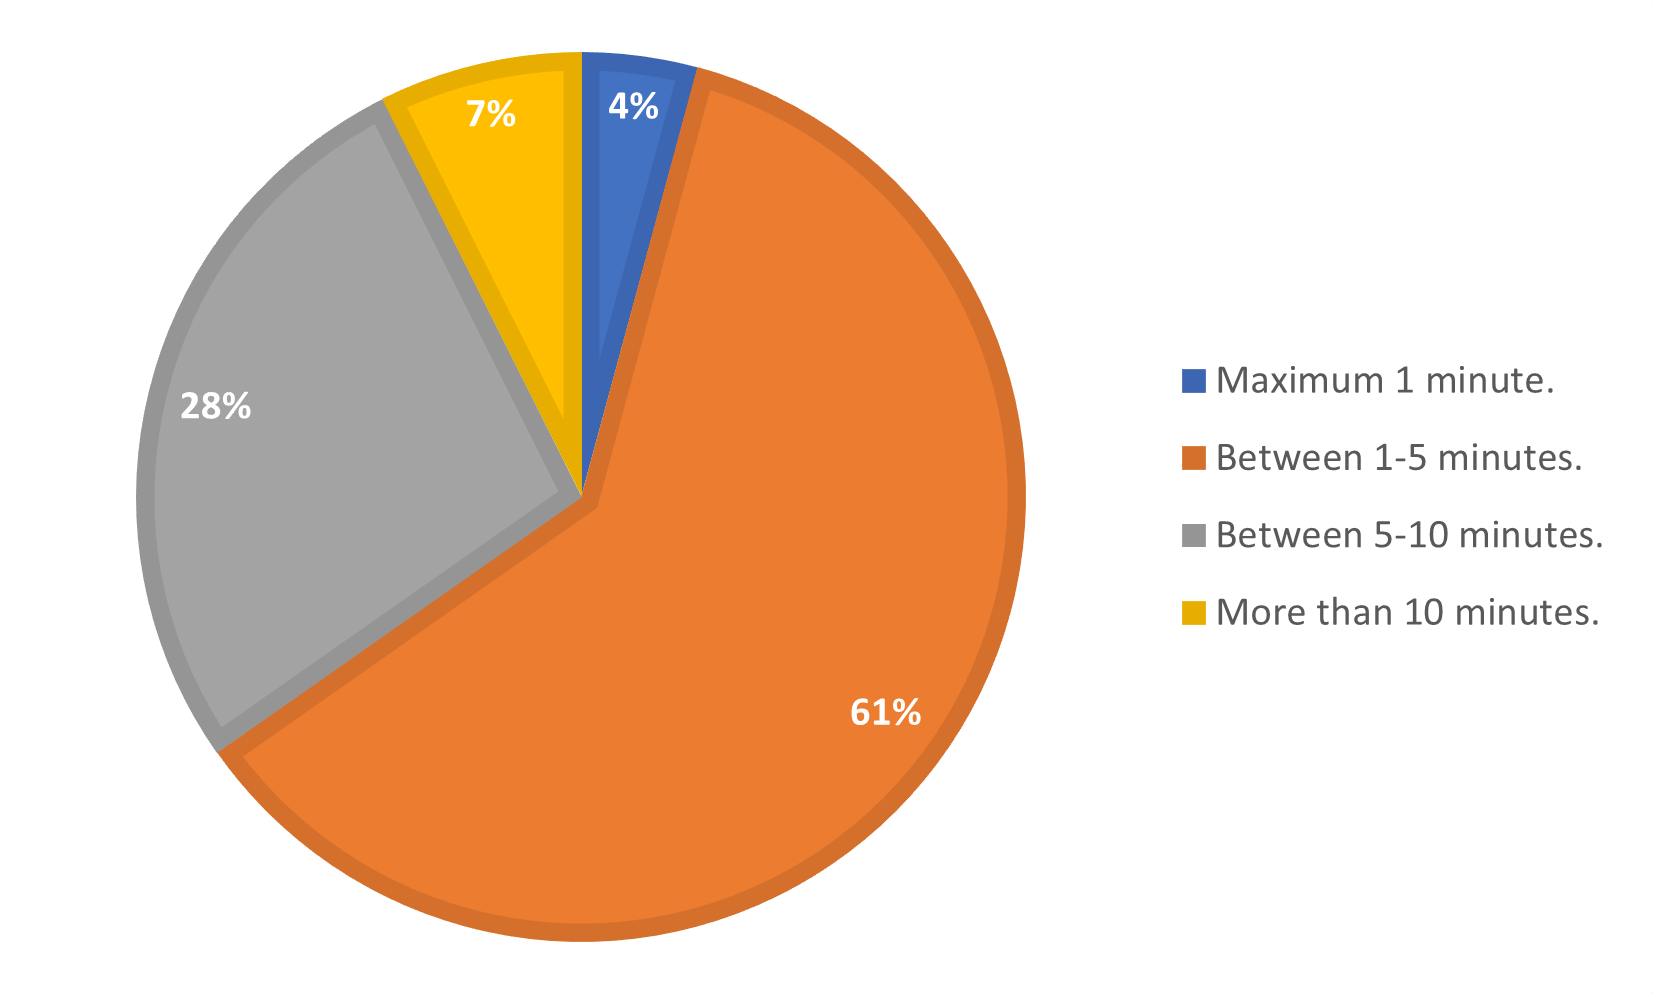
\includegraphics[height=0.25\textheight]{figures/charts/survey/feedback_time.png}
        \caption{The average time taken to complete a feedback questionnaire}
        \label{3:fig:feedback_time}
    \end{figure}

    ~

    Statistics about the reasons that sometimes determine students not to give feedback can be observed in figure \ref{3:fig:reasons_no_feedback}. Therefore, it is quite worrying that over \textbf{70\%} of students cannot identify ideas for improvement and over \textbf{65\%} consider it  is pointless, because it will not be examined.
    
    On the contrary, it is gratifying that under \textbf{1\%} of students mentioned they do not complete such questionnaires due to laziness, oblivion, or not being rewarded.
    
    \clearpage
    
    \begin{figure}[ht]
        \centering
             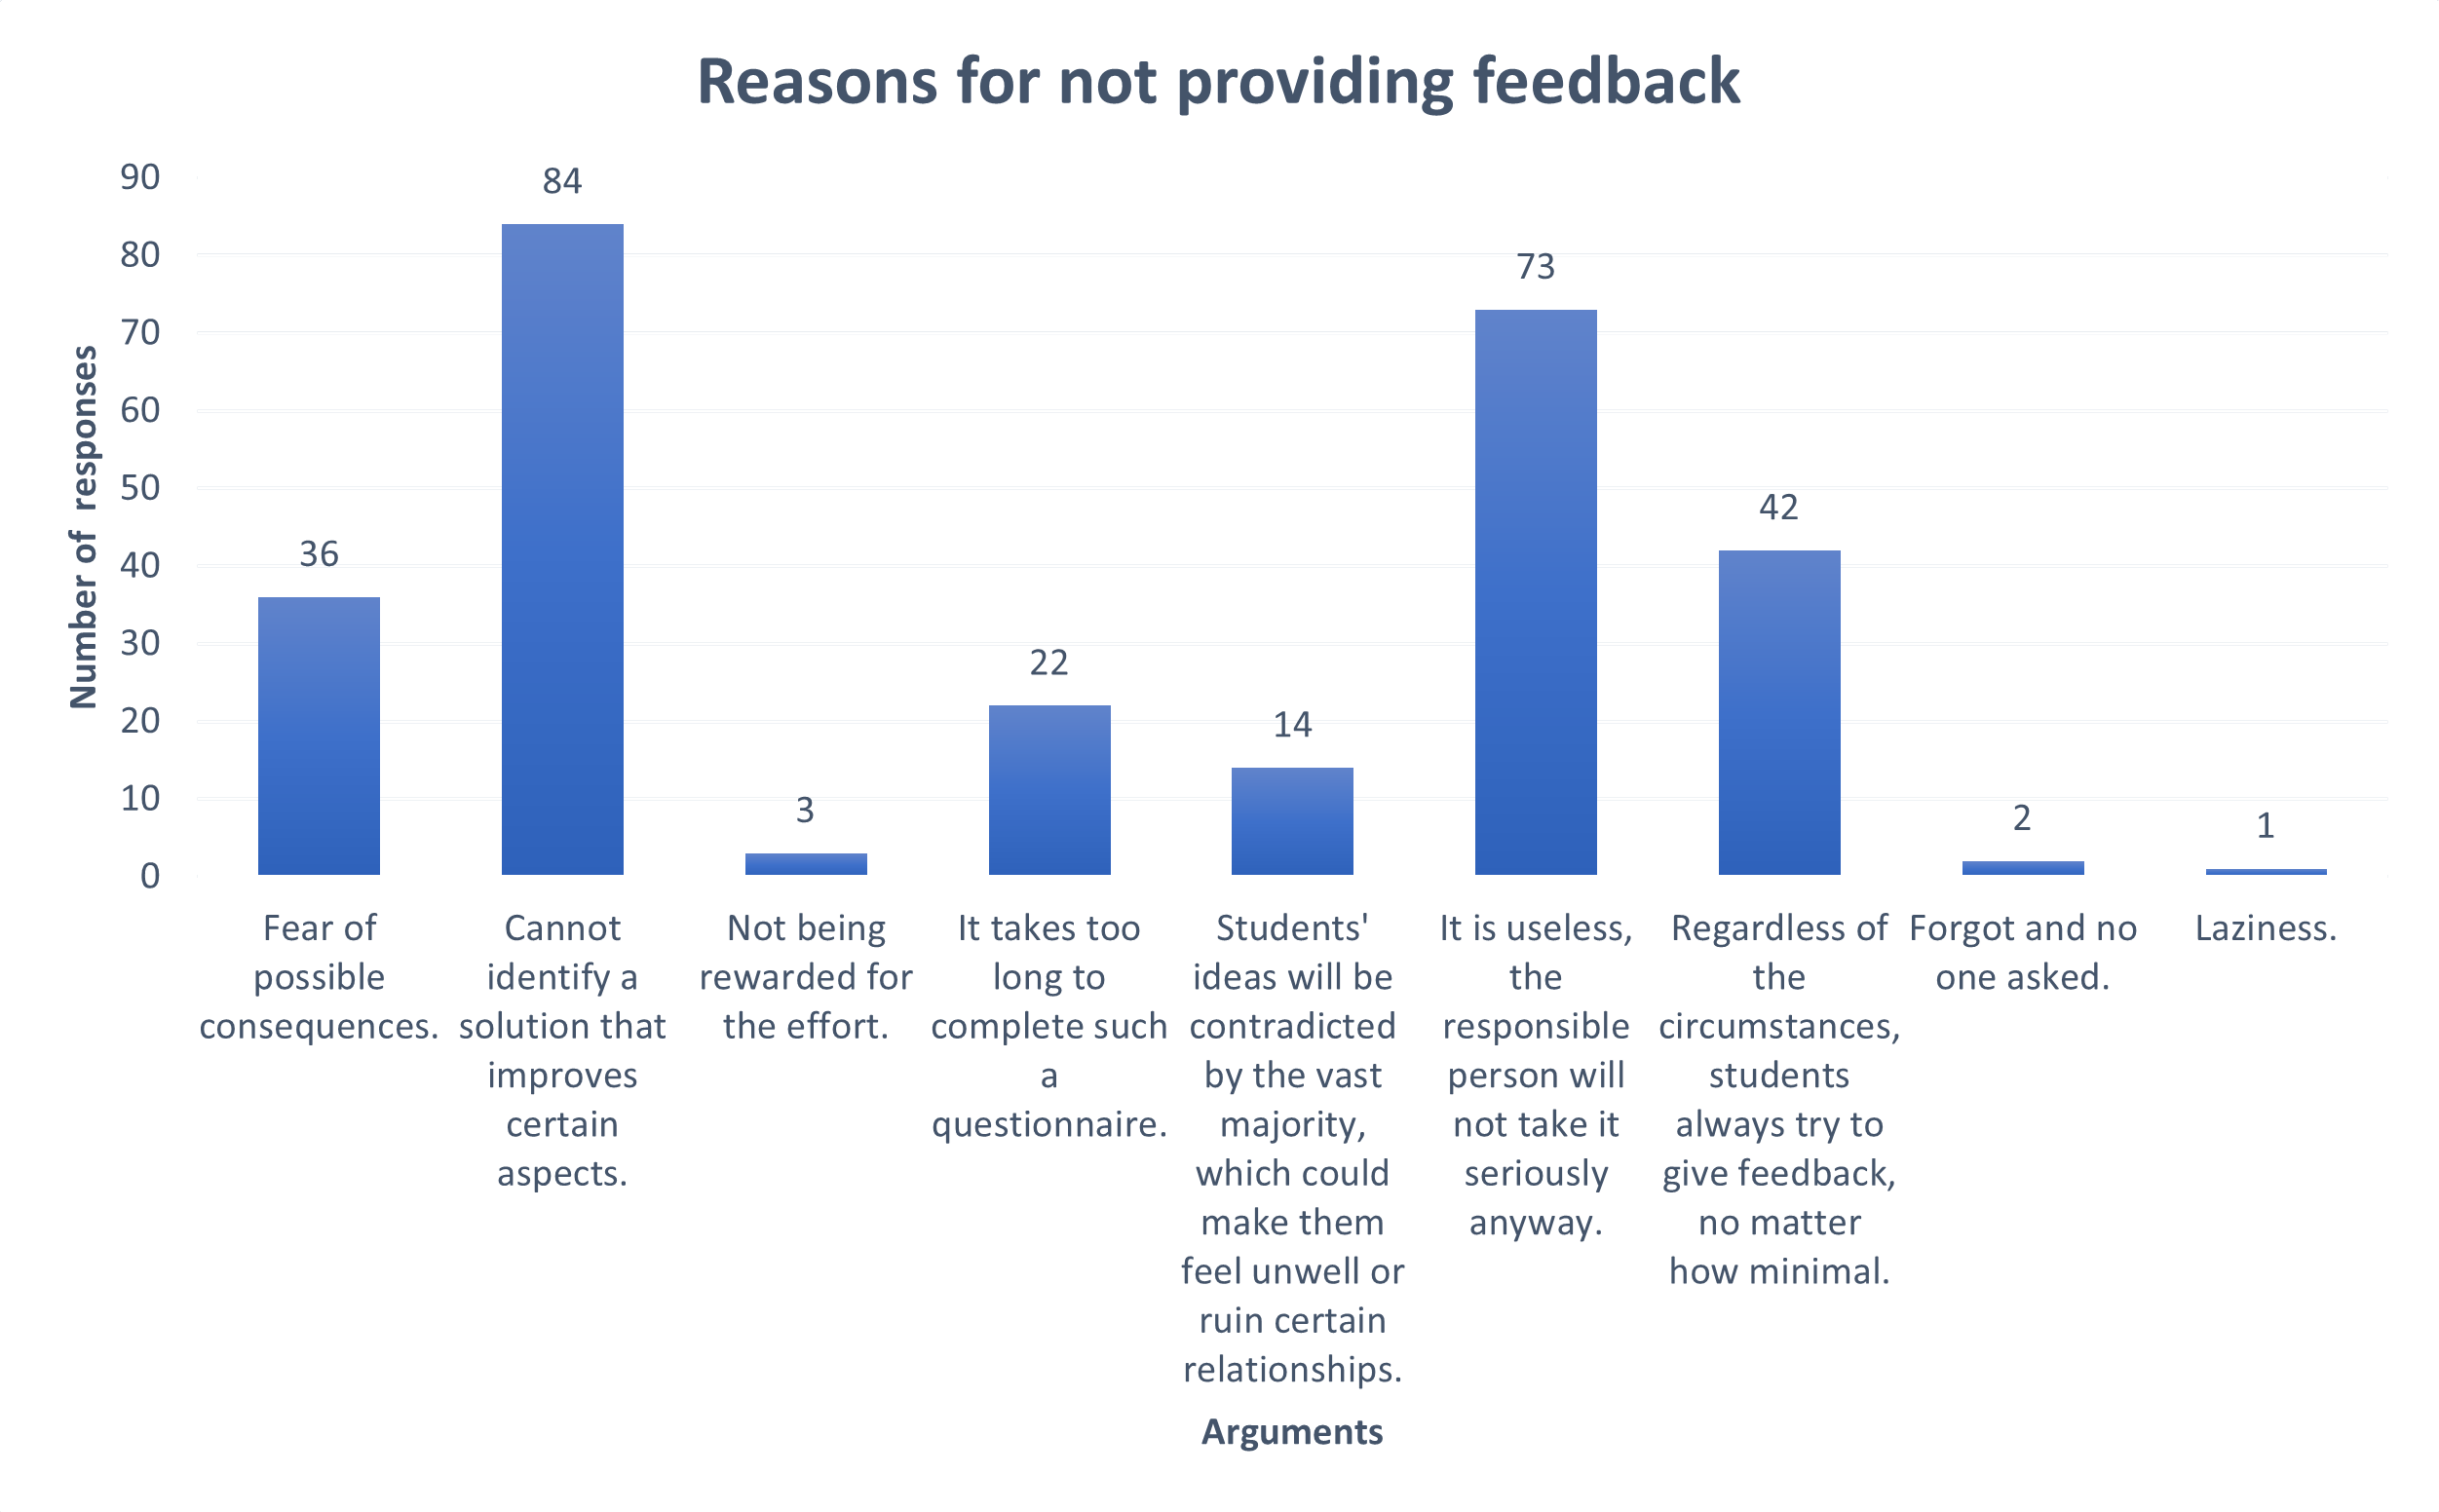
\includegraphics[height=0.4\textheight]{figures/charts/survey/reasons_no_feedback.png}
        \caption{Reasons for not providing feedback}
        \label{3:fig:reasons_no_feedback}
    \end{figure}
    
    Moreover, the vast majority of students said they were interested in finding out what others thought about specific ideas (fig. \ref{3:fig:feedback_interest_barchart}). This feature does not exist on the official courses platform, Moodle. Therefore, it is utterly non-transparent in terms of the finality of the feedback.
    
    \begin{figure}[ht]
        \centering
             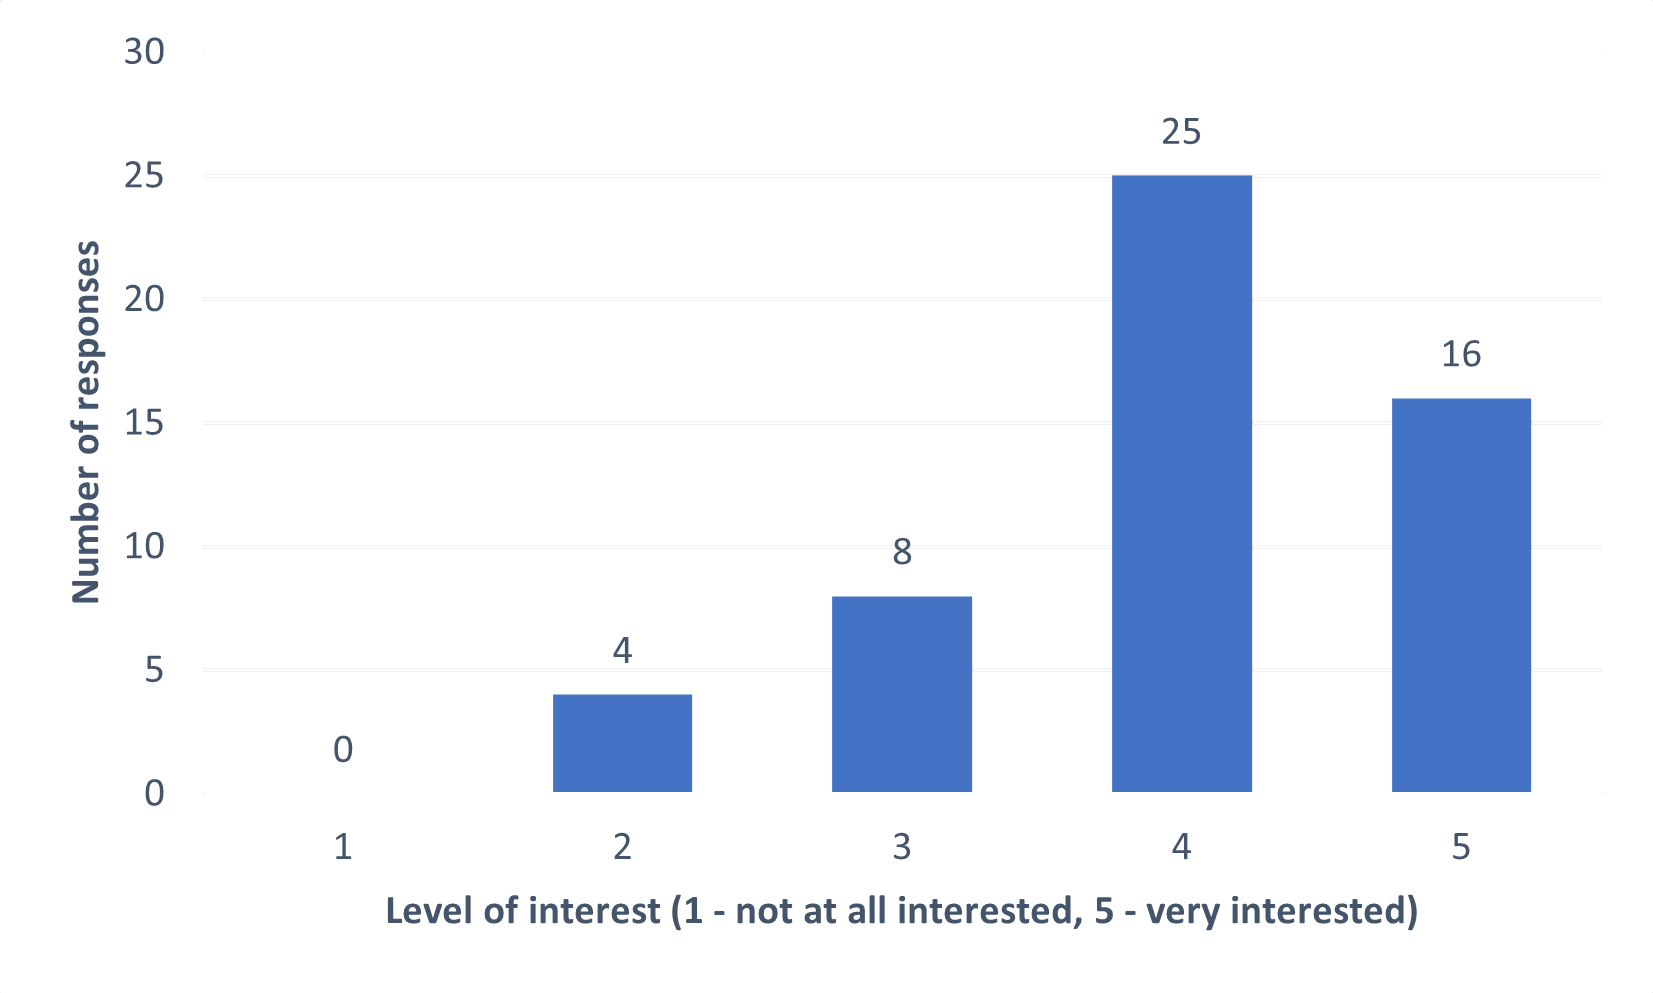
\includegraphics[height=0.24\textheight]{figures/charts/survey/feedback_interest_barchart.png}
        \caption{Interest of students in the opinions of others}
        \label{3:fig:feedback_interest_barchart}
    \end{figure}
    
    \clearpage
    
    \begin{figure}[ht]
        \centering
             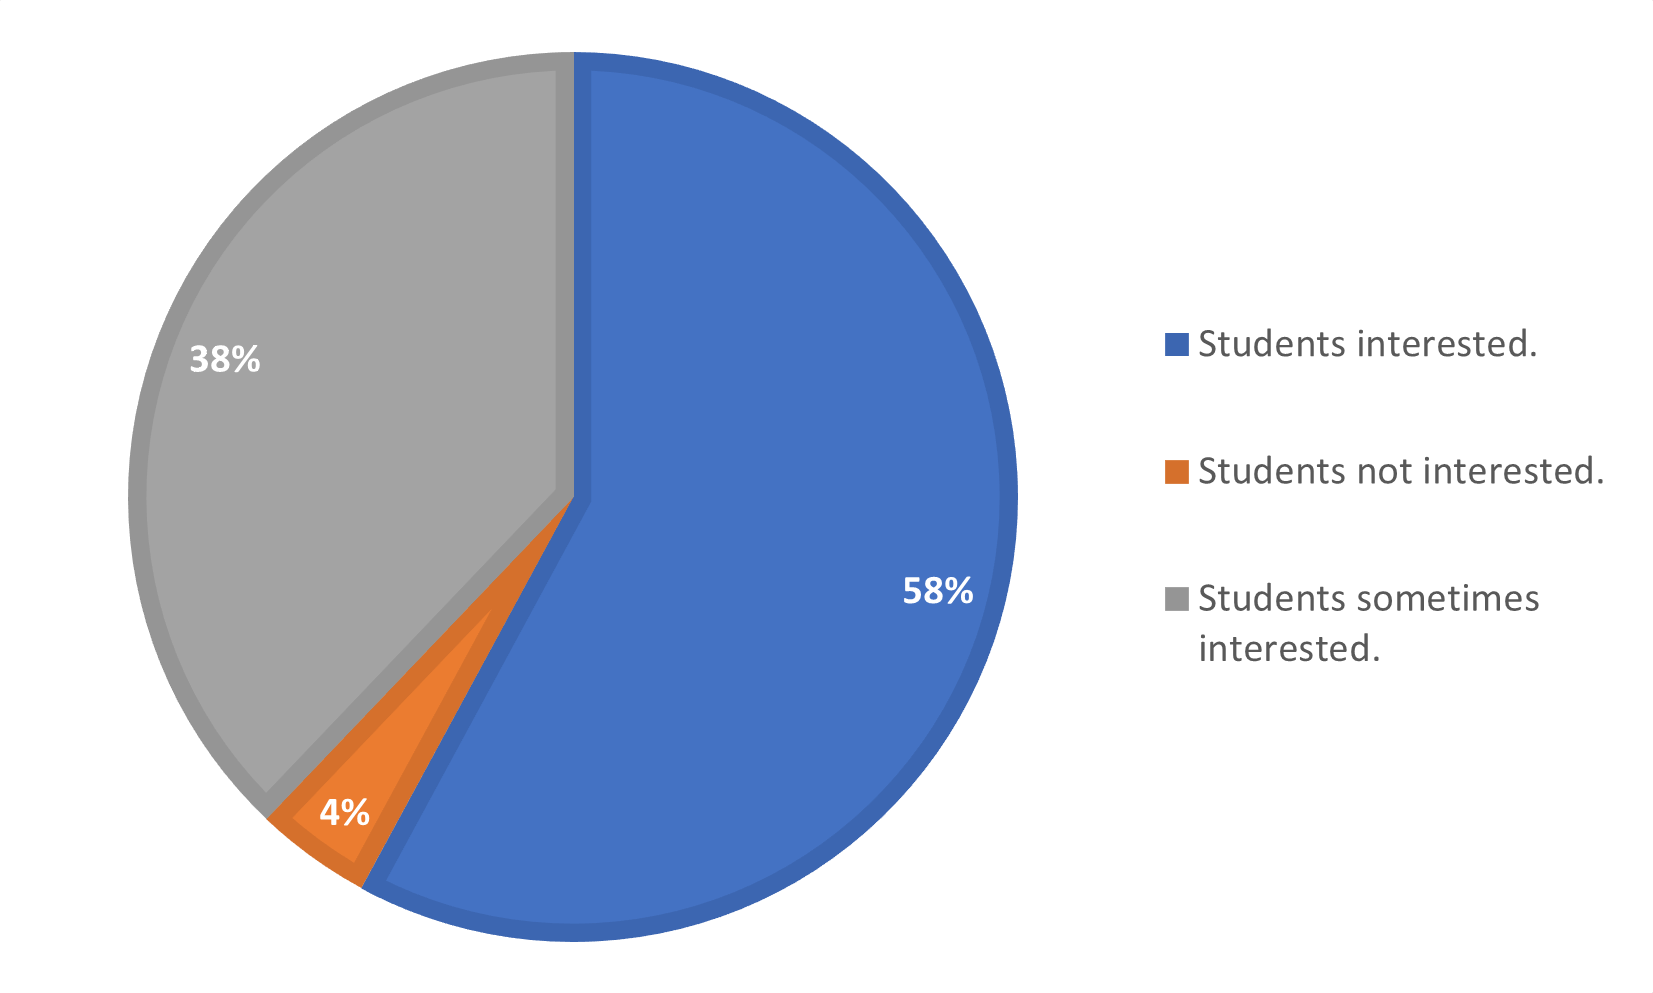
\includegraphics[height=0.22\textheight]{figures/charts/survey/overall_interest.png}
        \caption{Overall interest of students in the opinions of others}
        \label{3:fig:overall_interest}
    \end{figure}
    
    However, even if they do not provide feedback, students still seem to be interested in the ideas of others.
    
	Last but not least, we found that a very high percentage of answers from students specify that they want to know more details corresponding to tips and tricks, the amount of homework received and the effort required to solve it, and whether to choose a class as optional or not:
	
	\begin{figure}[ht]
        \centering
             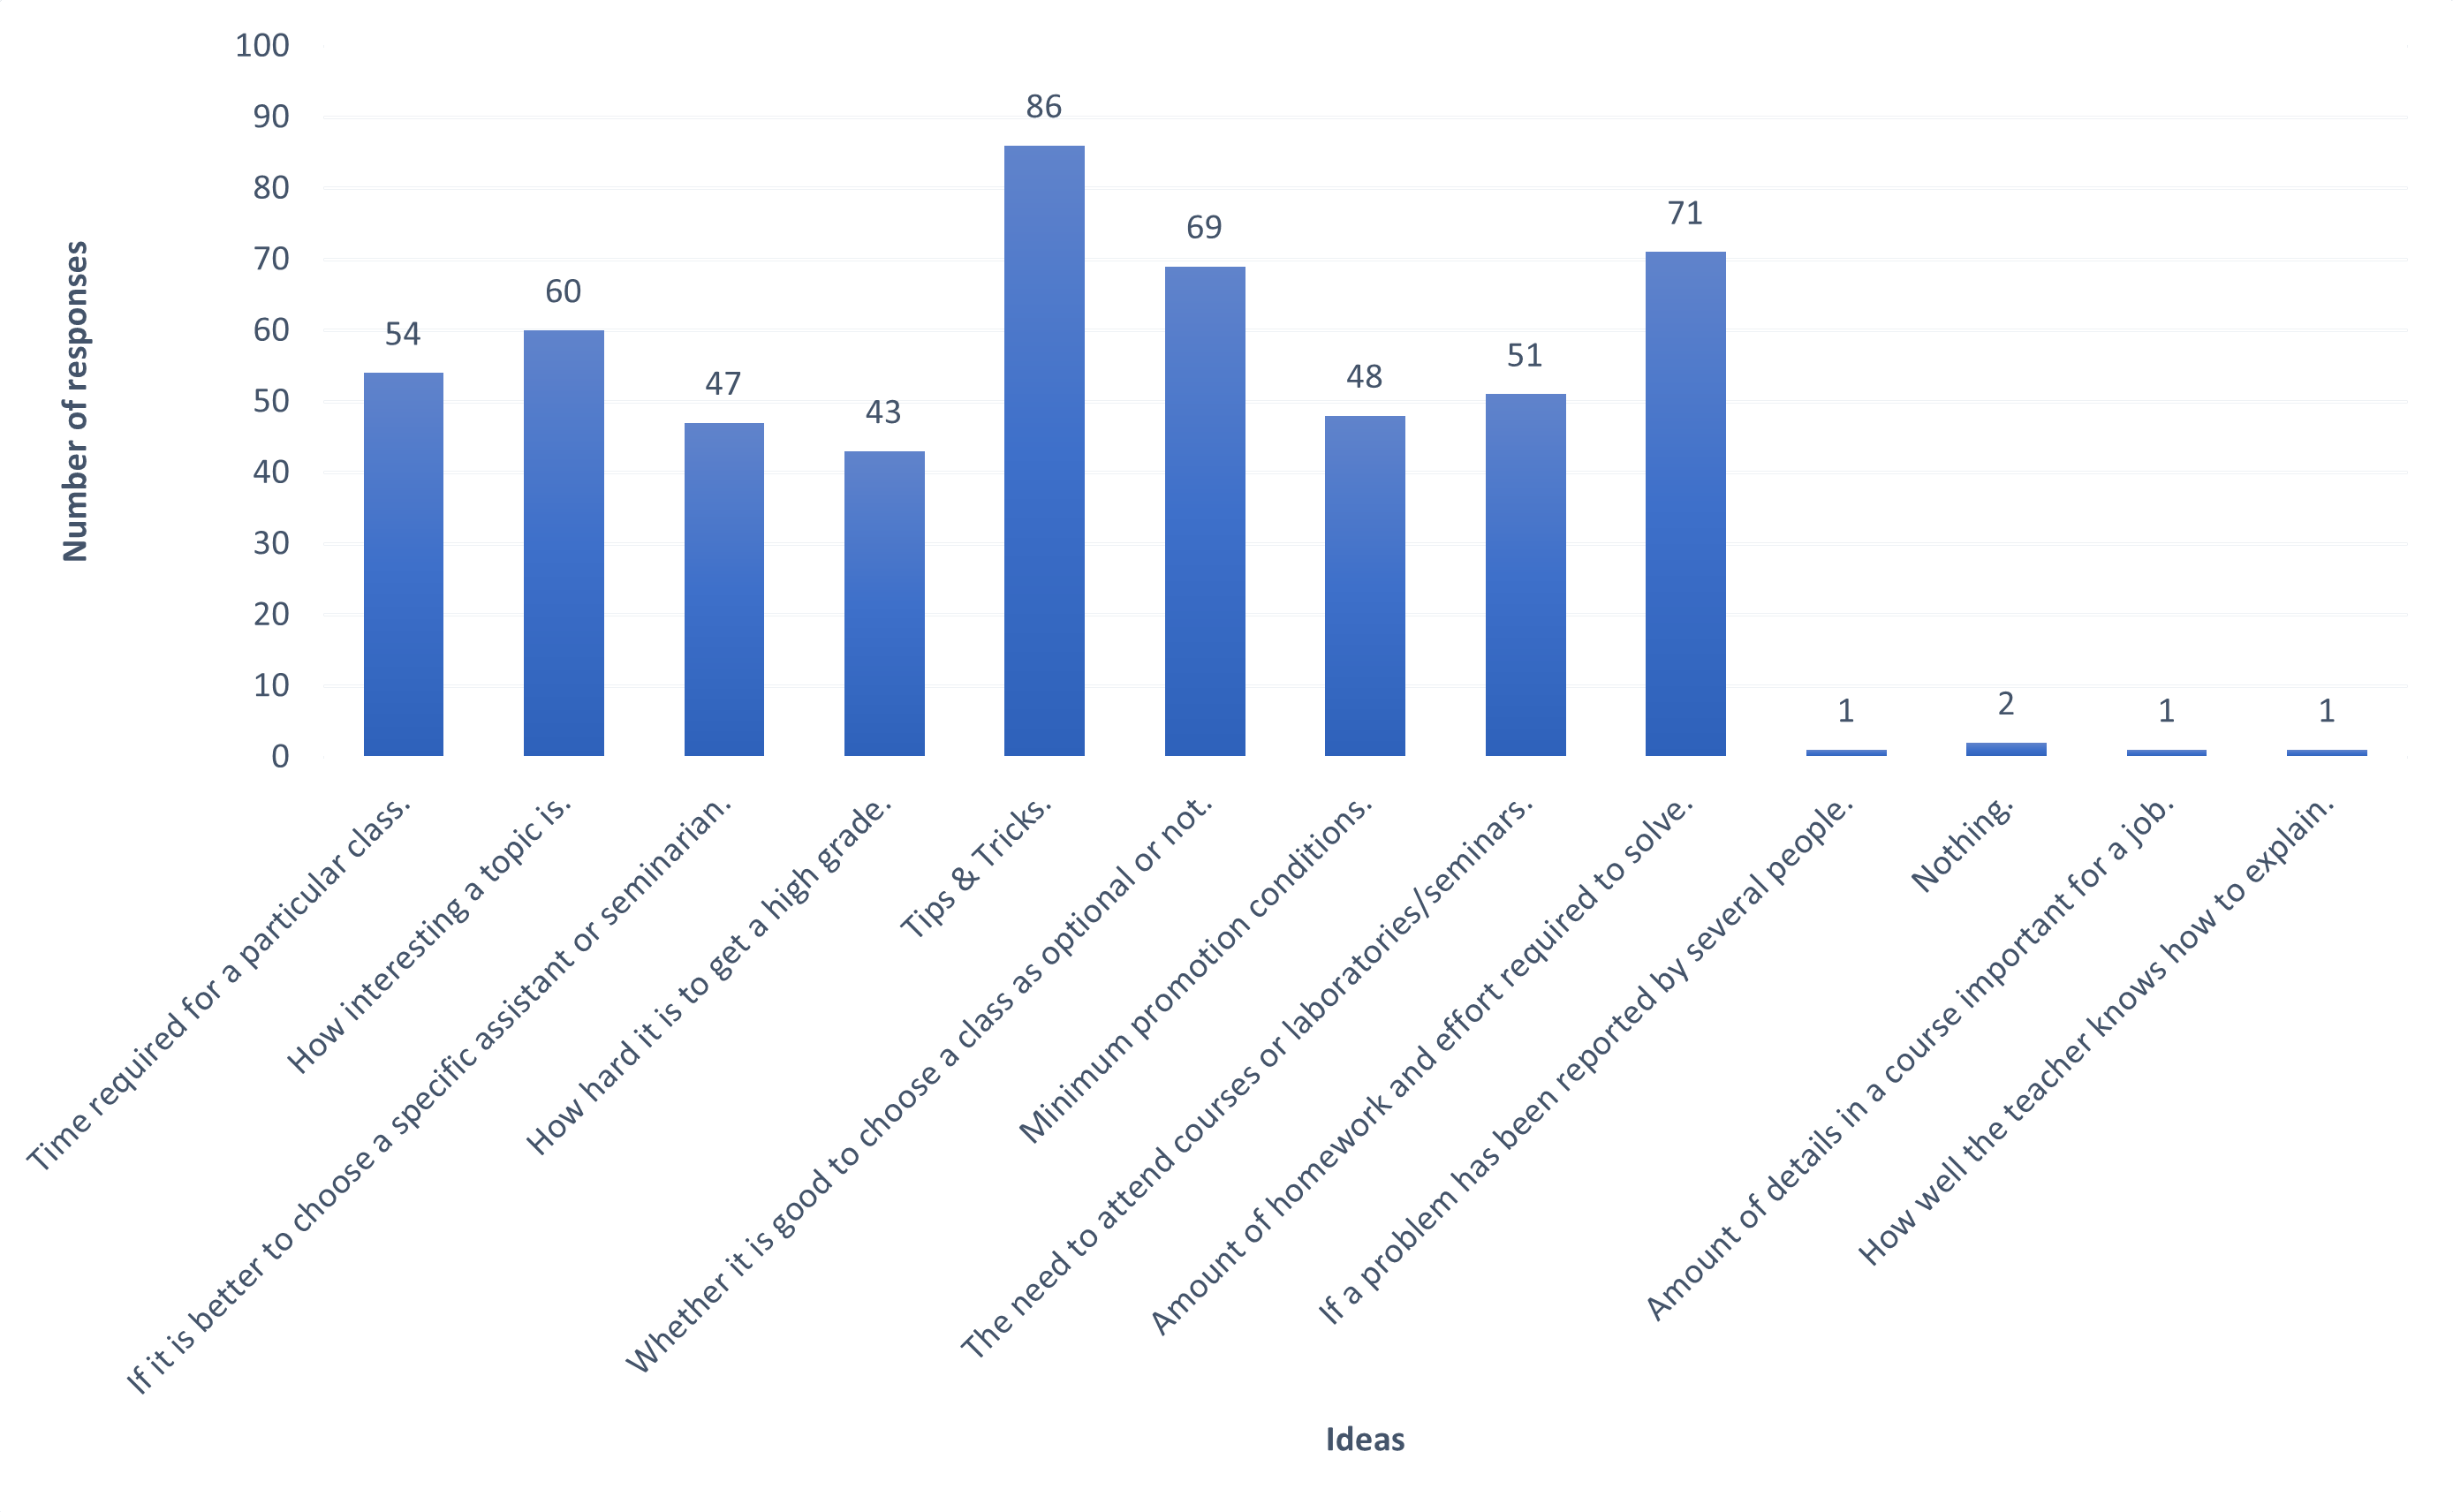
\includegraphics[height=0.42\textheight]{figures/charts/survey/students_interest.png}
        \caption{Main points of interest for students}
        \label{3:fig:students_interest}
    \end{figure}


    

